\section{Multilinguale Spracherkennung}
Die Kernidee der mehrsprachigen Spracherkennung ist bei den verschiedenen Architekturen dieselbe. Die Hidden-Layer des Deep Neural Networks können als ein intelligentes Merkmalsextraktionsmodul betrachtet werden, welches aus mehreren Quellsprachen trainiert wird. Nur die Ausgabeschicht liefert eine direkte Übereinstimmung mit den relevanten Klassen. So lassen sich die Extraktoren für eine Reihe verschiedener Sprachen gemeinsam nutzen. Wie im vorherigen Kapitel bereits erläutert wurde, lässt sich somit besonders das Problem beim Lernen der tiefen neuronalen Netze entgegenwirken. Diese lassen sich aufgrund ihrer Parameter und dem sogenannten Backpropagation-Algorithmus langsamer trainieren als andere Modelle. Ein weiterer Vorteil, den dieser Ansatz bietet ist, dass auch mit Sprachen, die nur einen geringen Satz an markierten Trainingsdaten bietet, erlernt werden können, indem Elemente anderer Sprachen übertragen werden. Merkmale, die aus diesen neuronalen Netzen extrahiert werden, lassen sich kombinieren, um so die Erkennungsgenauigkeit zu verbessern [1].
Eine gemeinsame Nutzung wird ermöglicht, indem Phoneme gemeinsam genutzt werden. Phoneme sind als kleinste, bedeutungsunterscheidende Einheiten der Lautsprache definiert. Phoneme werden zur Repräsentation der Aussprache genutzt. Um obige Ansätze zu nutzen, müssen Beziehungen zwischen den akustischen Signalen der Sprachen erkannt werden. Jede Sprache besitzt dabei ihre eigenen Charakteristika. In der Sprachübergreifenden Erkennung gibt es einen Satz aus trainierten sowie untrainierten bzw. schlecht trainierten Phonemen, die erkannt werden müssen. Die Töne einer Sprache müssen mit einem ähnlichen bzw. dem ähnlichsten trainierten Ton einer anderen Sprache ersetzt werden. Beispielsweise gibt es den Ton /y/, welcher im Wort ‚süß‘ vorkommt. Wenn ein System nun mit der deutschen Sprache genutzt wird, welches nur in anderen Sprachen trainiert wurde, muss der ähnlichste Sound zu /y/ gefunden werden [5]. So lassen sich phonetische Klassen aus mehreren Sprachen unterscheiden. Ein Transfer des Modells ist trivial. Es wird leidglich eine neue Softmax-Schicht angelegt und trainiert. Die Softmax-Funktion wird zur Klassifikation verwendet [6]. Die Ausgabenkoten dieser Schicht entsprechen dann den Senonen der Zielsprache. Senonen beschreiben lediglich das Betrachten des lautlichen Kontextes der einzelnen Phoneme und stellen gebundene Triphonzustände dar [1]. Die Kontexte können komplex sein [7]. 
Die Softmax-Schicht wird nur auf die entsprechende Sprache trainiert. Weitere Verbesserungen lassen sich erzielen, indem das gesamte Netzwerk zusätzlich auf die neue Sprache abgestimmt wird. Ein solche Architektur ist in Abbildung (…) illustriert. Sie zeigt die gemeinsam genutzten Schichten, die die Merkmale extrahieren sowie die unterschiedlichen Input-Datensätze. Jede Sprache hat ihre eigene Softmax-Ebene. Mit der Softmax-Funktion lassen sich hier die Zustände des akustischen Modelles vorhersagen bzw. entsprechende Wahrscheinlichkeiten schätzen. Wird ein neuer Datensatz in das System gegeben, werden nur die sprachspezifische Schicht sowie die Hidden Layer angepasst. Andere Softmax-Schichten bleiben intakt. Nach dem trainieren der fünf Sprachen ist das System in der Lage diese fünf Sprachen zu erkennen. Die Erweiterung um eine Sprache ist trivial. Kommt eine weitere Sprache hinzu, wird leidglich eine neue Softmax-Ebene an das vorhandene Netzwerk angefügt und trainiert [1]. 

\begin{figure*}[h!]
	\centering
	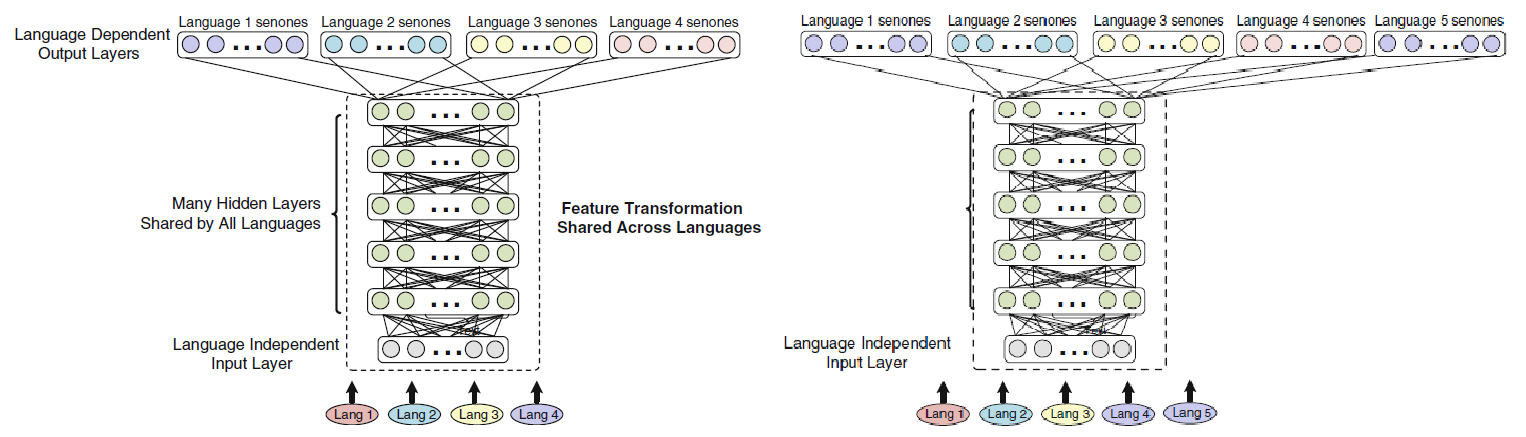
\includegraphics[width=1.0\linewidth]{images/shared_hidden_layer}
	\caption{Hinzufügen einer neuen Sprache  \cite{GonzalezDominguez.2015}} %Generelle
	\label{fig:topology}
\end{figure*}

Ein Vergleich eines monolingualen Deep Neural Networks und eines multilingualen Deep Neural Networks ist in Tabelle (…) aufgeführt. Das monolinguale Netzwerk wurde hierbei nur mit der entsprechenden Sprache trainiert, während das multilinguale System mit allen vier Sprachen trainiert wurde. Dabei wird die prozentuale Wortfehlerrate (Word error rate, WER) angegeben. Es ist zu erkennen, dass das multilinguale System das monolinguale in allen Sprachen übertrifft. Diese Verbesserung ist dem sprachübergreifenden Wissen zuzuschreiben [1]. 

\begin{table*}[h!]
	\begin{tabular}{lllll}
		& FRA             & DEU           & ESP           & ITA             \\
		Test set size (words) & 40k             & 37k           & 18k           & 31k             \\
		Monolingual DNN WER   & 28.1\%          & 24.0\%        & 30.6\%        & 24.3\%          \\
		Mulitlingual DNN WER  & 27.1\% (-3.6\%) & 22.7 (-5.4\%) & 29.4 (-3.9\%) & 23.5\% (-3.3\%)
	\end{tabular}
	\centering
	\caption{Relative Wortfehlerrate}
	\label{my-label}
\end{table*}

In [2] wurden eine Reihe weiterer Versuche durchgeführt, um die Wirksamkeit eines solchen Systems zu evaluieren. Dabei wurde zwei verschiedene Zielsprachen verwendet. Zum einen das amerikanische Englisch, welches phonetisch nahe an den europäischen Sprachen der Tabelle (…) liegt und Mandarin-Chinesisch, welches weit von den europäischen Sprachen entfernt ist. 
Die tatsächliche Erkennung der Sprache ist dabei trivial. Die Schallwellen, die beim Sprechen produziert werden, lassen sich über einen elektroakustischen Wandler (Mikrophon) in ein elektrisches Signal umwandeln. Dieses elektrische Tonsignal wird daraufhin in Zahlen bzw. Bits konvertiert (sampling) und über Vorverarbeitung entsprechend aufbereitet, um es in ein neuronales Netz zu speisen [4]. Beim genauen Vorhersagen des gesprochenen kommt die Sprachidentifikation ins Spiel, durch welche Wörter ausgeschlossen werden, die ebenfalls in Frage kommen, allerdings zum Wortschatz einer anderen Sprache gehören. Hat ein System z.B. die deutsche Sprache erkannt, wird für das Wort „Hello“ immer „Hallo“ vorhergesagt, da dies naheliegender ist. Es wird hier mit statistischen Modellen gearbeitet, um anzugeben mit welcher Wahrscheinlichkeit welches Wort vorkommt oder aufeinander folgen können. Dabei gibt es verschiedene Lösungsansätze, um das gesprochene vorherzusagen. Oft werden tiefe neuronale Netze in Verbindung mit Hidden Markov-Modellen eingesetzt. Diese hybriden Systeme werden in der Literatur oft untersucht und beschrieben. Ein allerdings leistungsfähigeres Modell bieten die Recurrent Neural Networks. Diese Form von neuronalen Netzen werden heutzutage eingesetzt und erreichen hohe Genauigkeiten [1].


\section{Recurrent Neural Networks}
Im Bereich der Spracherkennung werden heutzutage sogenannte Recurrent Neural Networks eingesetzt, durch welche die Netzwerke ihre Spracherkennungsgenauigkeit erreichen. Das Modell dieser Netze erlaubt gerichtete zyklische Verbindungen zwischen den Neuronen, wodurch es mit einem temporalen Verhalten ausgestattet wird. Recurrent Networks sind somit ideal zum Lernen von Datensequenzen geeignet. Sprache, also kontinuierliche Audiostreams fallen somit ebenfalls in das Anwendungsgebiet dieser Netzwerke. Diese Form von neuronalen Netzen unterscheidet sich grundlegend von dem Feed-Forward-DNN, da es nicht nur basierend auf Eingaben arbeitet, sondern auch auf interne Zustände zurückgreift. Diese internen Zustände speichern die vergangenen Informationen in der zeitlichen Reihenfolge, in welcher diese verarbeitet wurden. Somit ist ein RNN deutlich dynamischer, als ein Deep Neural Network, welches lediglich eine statische Eingabe-Ausgabe-Transformation durchführt. Dabei wird eine Erweiterung des Backpropagation-Algorithmus eingesetzt. Die Backpropagation-Through-Time-Methode sorgt für das Berechnen der Gradienten. Diese werden im Gegensatz zum Standard-Algorithmus über die einzelnen Zeitschritte aufsummiert. In dieser Erweiterung des Backpropagation, welche in Recurrent Neural Networks eingesetzt wird, werden lediglich die Parameter einzelnen Zeitschritte zwischen den Ebenen geteilt. In Abbildung (…) ist ein vereinfachtes Modell illustriert [1].

\begin{figure*}[h!]
	\centering
	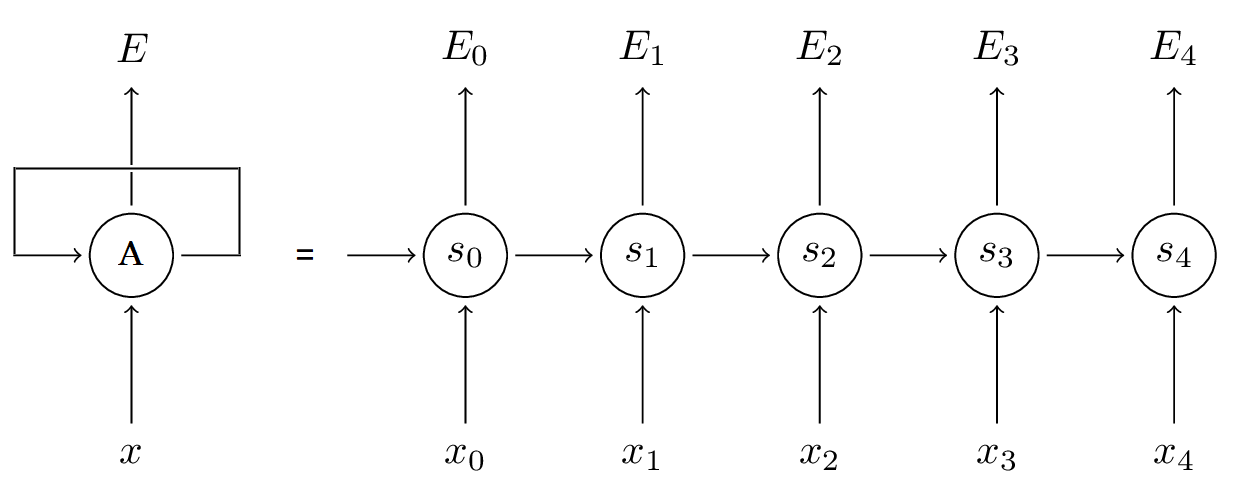
\includegraphics[width=0.5\linewidth]{images/rnn}
	\caption{Modell des Recurrent Neural Network  \cite{GonzalezDominguez.2015}} %Generelle
	\label{fig:topology}
\end{figure*}

Die Abbildung zeigt eine Folge von Iterationen. Der Input ist in obiger Darstellung x, s bezeichnet den Schritt und E den Hidden State, welcher sich beim Eingeben des Inputs ergibt. Ein Recurrent Network gibt somit nicht nur den Input an die nächste Iteration, sondern Input sowie den resultierenden Zustand E. Somit beeinflussen die vorhergehenden Schritte die folgenden. Dies führt zu einem Problem -dem Verschwinden von Information bzw. dem Vanishing Gradient Problem, welches sich dadurch ergibt, dass RNNs nicht in der Lage sind, auf Informationen zurückzugreifen, die weit in der Vergangenheit liegen.
Wenn eine Datensequenz lange ist und das System versucht die gesagten Worte vorherzusagen, kann es sein, dass der Kontext bereits vergessen wurde und eine inkorrekte Vorhersage stattfindet. Somit kommt eine erweiterte Form des RNNs zum Einsatz. Dieses wird Long-Short-Term-Memory (LSTM) genannt und erzielt enorm gute Ergebnisse in automatischen Spracherkennungssystemen [1][3]. 
Diese Netzwerke sind somit in der Lage anhand des Kontextes zukünftige Wörter vorherzusagen und so ihre Genauigkeit zu erhöhen.  Auch mit verrauschten Aufnahmen oder schlechteren Bedingungen beim Aufnehmen des Gesprochenen kann diese Form von Netzwerken bessere Ergebnisse erzielen. 
Aufgrund dessen wurden LSTM-Netzwerke entwickelt, die zur Lösung des Problems beitragen. Dabei werden Recurrent Neural Networks mit einer Speicherstruktur erweitert, was zur namensgebenden Lang-Kurzzeit-Speicherung führt. Diese erlauben die Erkennung zeitlich ausgedehnter Muster und das Erkennen von Zusammenhängen von zeitlich getrennten Ereignissen. Somit eignen sich die Netzwerke um Zeitreihen zu verarbeiten und vorherzusagen. Sogar, wenn zwischen wichtigen Ereignissen sehr lange Verzögerungen liegen, die eine unbekannte Länge aufweisen. Auch bei der Erlernung geräuschverzerrter und hallender Sprachmerkmale kann dieses Modell genutzt werden [1]. 
Die grundsätzliche Idee dabei ist es über elementweise Multiplikationen den Informationsfluss in dem Netzwerk zu steuern. Es kann als komplexe und intelligente Netzwerkeinheit betrachtet werden, welche Informationen über einen langen Zeitraum speichern kann. Dies wird durch die Gating-Struktur erreicht, die bestimmt, wann die Eingabe signifikant genug ist, um sich daran zu erinnern, wann sie sich die Information weiter merken oder vergessen sollte und wann sie die Information ausgeben sollte. Dies geschieht über verschiedene Gates innerhalb einer LSTM-Zelle (…). Ein Gate ist dabei nichts weiter, als eine Reihe von Multiplikationen bzw. Matrixoperationen [1].
Das System ist somit in der Lage aus dem Kontext heraus genaue Vorhersagen zu treffen, wodurch Spracheerkennung deutlich präziser wird. 
Allerdings ist es selbst heute nicht möglich das Spracherkennungsproblem allgemein zu lösen. Spracherkennungssysteme werden somit nur für bestimmte Anwendungsfälle oder Szenarien konzipiert. Mit einer solchen Spezialisierung auf entsprechende Anwendungsgebiete können zum einen höhere Genauigkeiten erreicht werden und zum anderen wird nicht so viel Rechenleistung und Speicher benötigt [4]. Vor allem bei der multilingualen Spracherkennung besteht die Schwierigkeit Gemeinsamkeiten verschiedener Sprachen zu nutzen, um Sprachen mit wenig Trainingsdaten mit einer ausreichenden Genauigkeit anzubieten. Es gilt die Sprachen zu finden, die zur besten Erkennungsleistung der neuen Sprache führen. Dabei müssen Beziehungen zwischen den Sprachen erkannt werden. Problematisch ist auch, dass gleiche Phoneme je nach Sprecher, Sprache etc. variieren, was dazu führt, dass Phoneme nur im Kontext betrachtet werden (Triphone). 